\documentclass[17pt]{beamer}
\usepackage{graphicx}
\usepackage{tikz}
\usepackage{tikz-cd}
\usepackage{amsfonts}
\usepackage{amssymb}
\usepackage{amsmath}
\usepackage{amscd}
\usepackage{amsthm}
\usepackage{bbm}
\usepackage{fourier}
\usepackage[utf8]{inputenc}
\title{Ontology for Liberals}
\author{Hans Halvorson}
\date{June 29, 2017}
\setbeamertemplate{navigation symbols}{}%remove navigation symbols
\usepackage{eucal}
\setbeamercolor{normal text}{fg=black,bg=white}
\setbeamercolor{alerted text}{fg=red}
\setbeamercolor{example text}{fg=black}
\usepackage[absolute,overlay]{textpos}
\begin{document}
\def\2{\mathcal}
\def\7{\mathfrak}

%% primitive ontology

%% preference for configuration space representations -- L2(R) as
%% opposed to other Hilbert spaces

%% How far are you willing to take that?  Dedekind cuts vs Cauchy reals.

%% literal interpretation

%% signatures for STR

%% Hamiltonian vs Lagrangian

%% model isomorphism criterion

%% a way the world could have been --- Bohm with momentum

\begin{frame}

\maketitle 

\end{frame}

\begin{frame}

  % Bohr quote
  ``We not only believe the existence of atoms to be proved beyond a
  doubt, but also we even believe that we have an intimate knowledge
  of the constituents of the individual atoms.''
  

\end{frame}


\begin{frame}{An Alluring Idea}

  A well-defined \textbf{theory} must have a (primitive)
  \textbf{ontology}

  \bigskip i.e.\ an old-fashioned catalog of material objects 


\end{frame}
\begin{frame}

  \begin{description}
\item[good] classical particle mechanics, Bohmian mechanics
\item[bad] orthodox quantum mechanics, Copenhagen
\item[ugly] many worlds QM 
\end{description}

%% ?? WHAT's my segue here ??

\end{frame}


\begin{frame}

  \begin{itemize}
  \item The primitive ontology approach stresses the virtue of clear
    and unambiguous communication.
  \item But it runs the danger of \textbf{semantic fundamentalism}.
  \end{itemize}

  %% what do we mean here by fundamentalism?


  %% I know fundamentalism when I see it -- e.g. Christians arguing
  %% about whether women should be allowed to lead a church service.


\end{frame}

\begin{frame}

  \begin{itemize} \item \textbf{semantic fundamentalism:} drawing
    finer distinctions between theories than there are distinctions in
    the world.
  \item Examples
    \begin{itemize}
    \item Demanding that a theory be written in German instead of English.
    \item Demanding that we use polar coordinates instead of Cartesian
      coordindates.  
     \end{itemize}  \end{itemize}

\end{frame}



\begin{frame}{Main Questions}

  \begin{itemize}
    \item When are \textbf{two} descriptions of reality \textbf{equivalent} to
      each other?
    \item What disputes are worth having?
    \item What kind of distinctions does the world care about?    
  \end{itemize}

\end{frame}





\begin{frame}{left wing views}

  %% empirical equivalence

  \begin{itemize}
  \item \textbf{empirical equivalence}: If two theories make the same
    predictions, then they're equivalent.
    % Other differences don't matter.
    %% Schrodinger vs Heisenberg
  \end{itemize}
  

\end{frame}  


\begin{frame}{left wing views}

  %% Diagram
  %% empirical equivalence

  \begin{center}
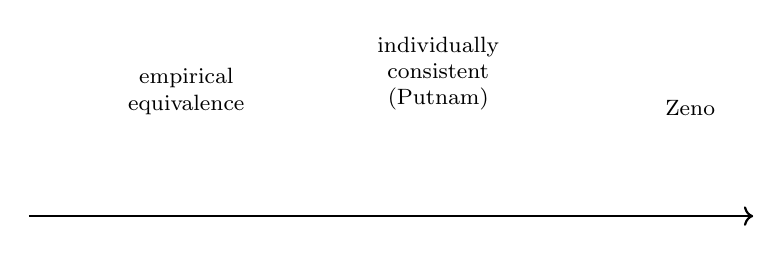
\begin{tikzpicture}[scale=0.8]
\tikzstyle{every node}=[font=\footnotesize]
\draw [-> ,thick ] (-1.5,0) -- (10,0);
\node[align=center, below] at (1,2.5) {empirical \\ equivalence};
\node[align=center, below] at (5,3) {individually \\ consistent \\
  (Putnam)};
\node[align=center, below] at (9,2) {Zeno};
\end{tikzpicture}
\end{center}

\end{frame}


\begin{frame}{moving to the right}

  %% start with views that might not seem so outlandish

  \begin{itemize}
   \item primitive ontology vs wave-function monism 
   \item wave mechanics vs matrix mechanics
   \item Hamiltonian mechanics vs Lagrangian mechanics
\end{itemize}

\end{frame}


\begin{frame}

  %% Now start making it look a bit more radical  
  %% How far should we go with this?

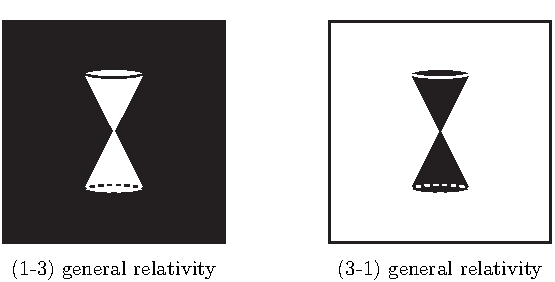
\includegraphics{solsorten.pdf}
  
    %% STR: 3+1 versus 1+3

\end{frame}



\begin{frame}{right wing views}


  \begin{center}
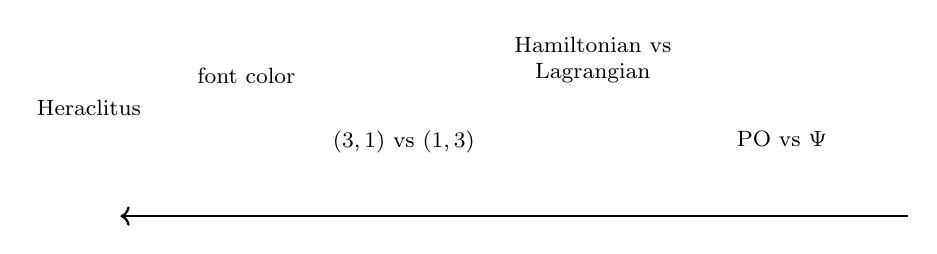
\begin{tikzpicture}[scale=0.8]
\tikzstyle{every node}=[font=\footnotesize]
\draw [<- ,thick ] (-4.5,0) -- (8,0);
\node[align=center, below] at (-5,2) {Heraclitus};
\node[align=center, below] at (-2.5,2.5) {font color};
\node[align=center, below] at (0,1.5) {$(3,1)$ vs $(1,3)$};
\node[align=center, below] at (3,3) {Hamiltonian vs \\ Lagrangian};
\node[align=center, below] at (6,1.5) {PO vs $\Psi$};

\end{tikzpicture}
\end{center}



\end{frame}

\begin{frame}{\normalsize Toward a clear account of theoretical
    equivalence}

%% got to start out with an idea of what kind of mathematical thing a
%% theory is

  \begin{itemize}
  \item Motivating idea: two theories are equivalent just in case they
    \textbf{say the same thing}.
  \item More precise: two theories are equivalent just in case they
    are \textbf{inter-translatable}.
   \end{itemize}


 \end{frame}

 \begin{frame}

   A first-order language consists of:
   \begin{itemize}
   \item logical symbols $\forall ,\exists ,\wedge ,\vee $, etc.\
   \item variables $x_1,x_2,\dots $
   \item a signature $\Sigma$ consisting of specific relation and
     function symbols.
   \end{itemize}

   \end{frame}

   \begin{frame}

     \begin{itemize}
       \item A \textbf{reconstrual} of $\Sigma$ into $\Sigma '$
         assigns to each relation symbol $R$ of $\Sigma$ a
         corresponding open-formula $\phi$ of $\Sigma '$.
       \item A reconstrual recursively generates a map from formulas
         of $\Sigma$ to formulas of $\Sigma '$.
       \item This map is a \textbf{interpretation} of $T$ into $T'$
         just in case $T\vdash \phi$ only if $T'\vdash \phi ^*$.
       \end{itemize}

 \end{frame}

\begin{frame}

Two theories $T$ and $T'$ are \textbf{homotopy equivalent}
      just in case there are interpretations $F:T\to T'$ and $G:T'\to
      T$ such that:
      \[
      \begin{array}{lll}  T & \vdash & \forall x(\phi
                                       (x)\leftrightarrow GF\phi (x))
        \\ 
      T' & \vdash & \forall x(\psi (x)\leftrightarrow FG\psi
                    (x)) \end{array} \] 

\end{frame}


\begin{frame}{Intuitive gloss}


  \begin{itemize}
  \item Each model $M$ of $T$ corresponds to a unique model $M'$ of
    $T$.
  \item $M$ and $M'$ are isomorphic --- i.e.\ have the same number of
    objects, and they stand in the same relations.
  \end{itemize}


\end{frame}


%% this is going to be the toughest part -- convincing them that this
%% account is too conservative

%% appeal to mathematical naturalness in notions of isomorphism?


\begin{frame}{Too conservative?}

  %% geometry picture
  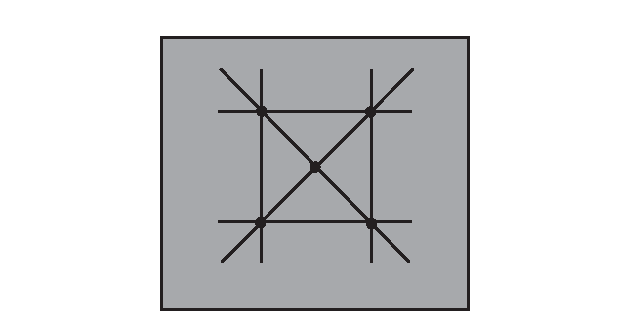
\includegraphics{affine1.pdf}

  %% but isn't this just pure math?  Is this relevant for the physical
%% world?

%% Lesson of relativity: not so easy to separate geometry from
%% material content

\end{frame}


\begin{frame}{\normalsize categorical equivalence}

$\mathrm{Mod}(T)$ consists of two kinds of things:

\begin{description}
\item[objects] models of $T$
\item[arrows] homomorphisms of models
\end{description}


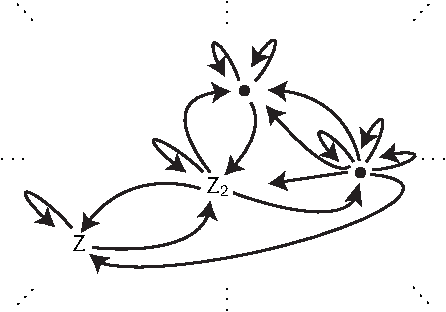
\includegraphics{grp1category.pdf}

%% to do: explain category of models

%% relations between models - embedding, symmetry, cover

%% *functor* takes models to models [but no restriction!], arrows to
%% arrows of the same type

%% $F$ is an equivalence -- two notions


\end{frame}

\def\3{\mathbf}


\begin{frame}{\normalsize categorical equivalence}

\begin{tabular}{l l l}
objects of $\3C$  & $\longmapsto$ & objects of $\3D$  \\
arrows of $\3C$  & $\longmapsto$ & arrows of $\3D$ \end{tabular}

\begin{itemize}
  \item preserves arrow structure  
  \item invertible, up to natural isomorphism
    \end{itemize}




\end{frame}








\begin{frame}{AZ equivalence}

  Generalized reconstrual: an $n$-ary relation symbol is mapped to an
  $nm$-ary formula
  \[ R(x_1,\dots ,x_n) \: \longmapsto \: \phi (\vec{y}_1,\dots ,
    \vec{y}_n) \]


\end{frame}

\begin{frame}{AZ equivalence}

  A homotopy equivalence between $T$ and $T'$ consists of a pair of
  reconstruals $F:T\to T'$, $G:T'\to T$, and connecting formulas
  $\eta$ and $\varepsilon$ such that:

  \[ \begin{array}{lll}

  T & \vdash & \forall x(\eta (x,\vec{y})\to (\phi (x)\wedge GF\phi
               (\vec{y})))  \\
  T' & \vdash & \forall x(\varepsilon (x,\vec{y})\to (\psi (x)\wedge
                FG\psi (\vec{y}))) \end{array} \]

\end{frame}            

\begin{frame}{Intuitive gloss}

  \begin{itemize}
  \item Each model $M$ of $T$ corresponds to a unique model $M'$ of $T'$.  
  \item But $M$ and $M'$ are \textbf{not} necessarily isomorphic.  
  \item Every object of $M'$ is a \textbf{logical construction} of
    objects of $M$, and vice versa.
  \end{itemize}


\end{frame}


%% do I have other examples besides the Tarski geometry example?  

\begin{frame}{the ideological spectrum}

\begin{center}
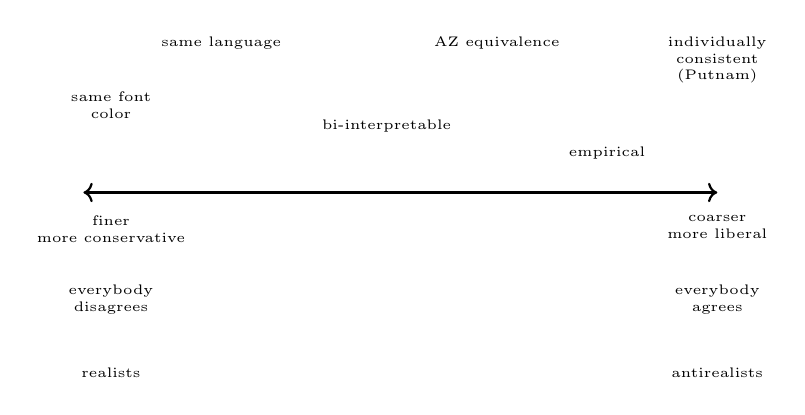
\begin{tikzpicture}[scale=0.7]
\tikzstyle{every node}=[font=\tiny]
\draw [<-> ,thick ] (-2.5,0) -- (9,0);
\node[align=center, below] at (-2,2) {same font \\ color};
\node[align=center, below] at (0,3) {same language};
\node[align=center, below] at (3,1.5) {bi-interpretable};
\node[align=center, below] at (5,3) {AZ equivalence};
\node[align=center, below] at (7,1) {empirical};
\node[align=center, below] at (-2,-0.25) {finer \\ more conservative};
\node[align=center, below] at (9,-0.25) {coarser \\ more liberal};
\node[align=center, below] at (9,3) {individually \\ consistent \\ (Putnam)};
\node[align=center, below] at (-2,-1.5) {everybody  \\ disagrees};
\node[align=center, below] at (-2,-3) {realists};
\node[align=center, below] at (9,-1.5) {everybody \\ agrees};
\node[align=center, below] at (9,-3) {antirealists};
\end{tikzpicture}
\end{center}




\end{frame}






\begin{frame}{Take home points}

\begin{itemize}
\item Our intuitive notion of theoretical equivalence calls for
  explication.
\item When explication uses math, we may be guided by internal
  mathematical standards --- which sometimes challenge naive
  intuitions.  (Example: notions of infinity)


\end{itemize}




\end{frame}


\begin{frame}{Take home points}

\begin{itemize}
\item You can be completely clear about, and committed to the
  correctness of one ontology --- while still conceding that there
  might be different, yet \textbf{equally correct}, ontologies.
\end{itemize}




\end{frame}  






\end{document}
